\documentclass[10pt]{article}

\usepackage{graphicx}

\newcommand{\mysection}[1]{\section{#1}\label{#1}}
\newcommand{\mysubsection}[1]{\subsection{#1}\label{#1}}
\newcommand{\mysubsubsection}[1]{\subsubsection{#1}\label{#1}}
\newcommand{\remark}[1]{[\emph{#1}]}

\begin{document}

\title{Ibis RMI}

\author{The Ibis Group}

\maketitle

\mysection{Java RMI}

Java applications typically consist of one or more threads that
manipulate a collection of objects by invoking methods on these
objects. Figure~\ref{normal-fig} shows an example, where a single application thread
has a reference to some interface which represents an object. The
thread and object are located in the same Java Virtual Machine (JVM),
and the thread can use normal method invocations on the interface to
manipulate the state of the object.

\begin{figure}[t]
\begin{center}
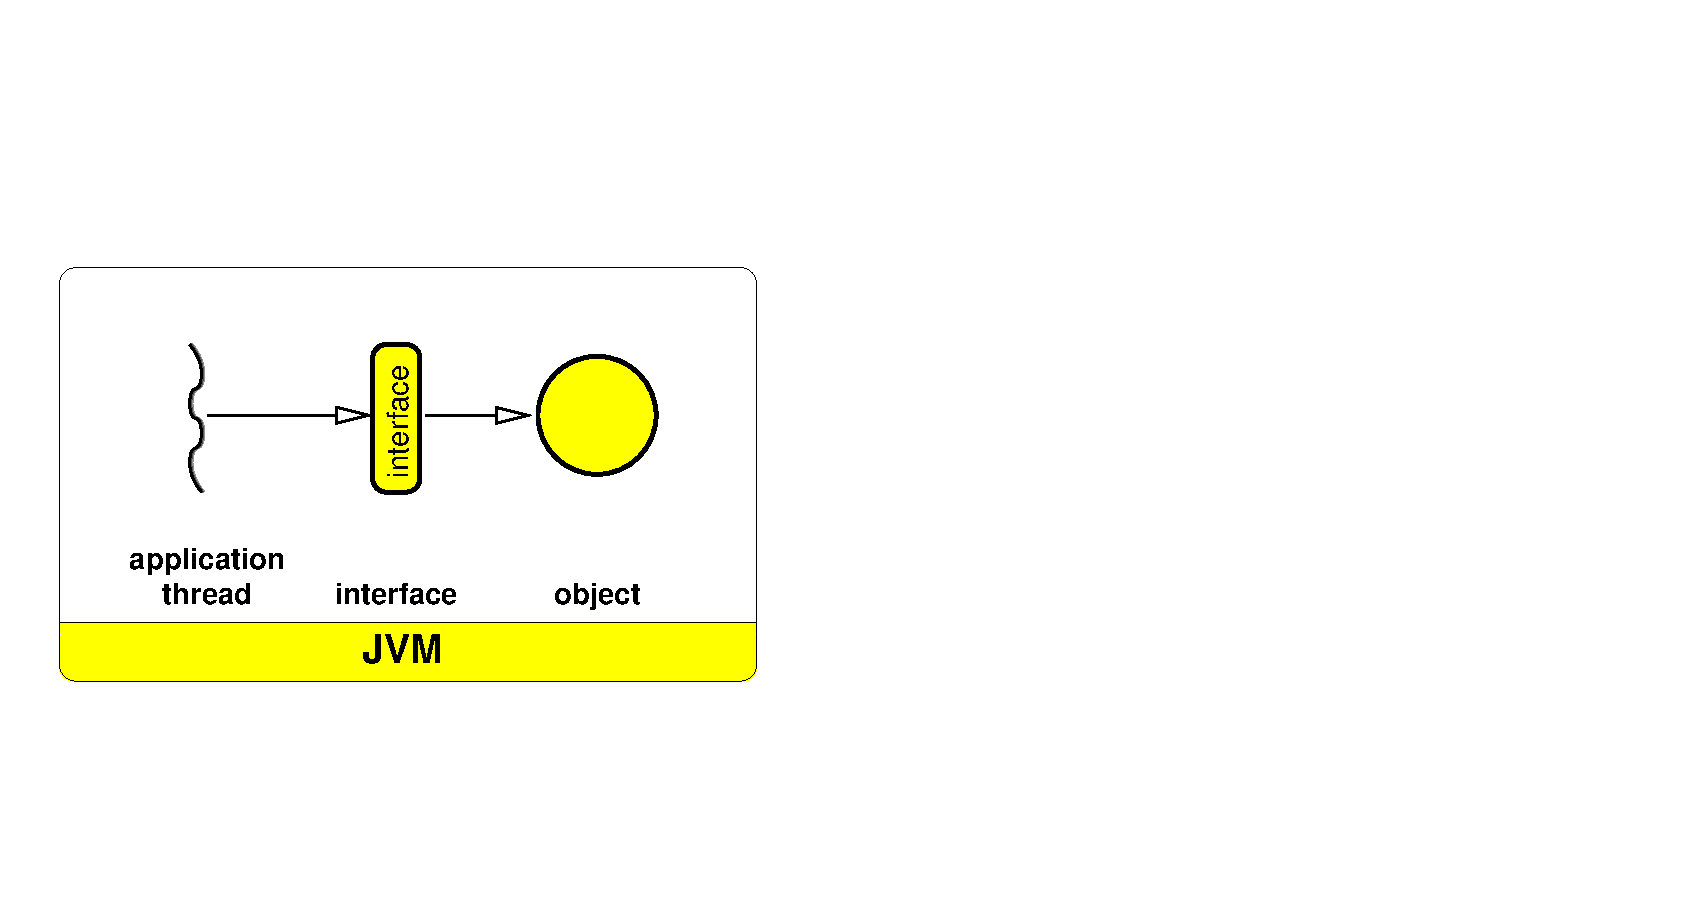
\includegraphics[width=0.7\textwidth]{normal.eps}
\end{center}
\caption{A normal invocation.}
\label{normal-fig}
\end{figure}

To turn the example of Figure~\ref{normal-fig} into a distributed RMI invocation,
some small modifications must be made to the program. The interface
must be turned into a remote interface by extending java.rmi.Remote,
and the object must be turned into a remote object by extending
java.rmi.UnicastRemoteObject. The rmic compiler, which is part of the
Java Developer Kit (JDK), can then generate the required communication
code. This code consist of two objects, a 'stub' and a 'skeleton', as
shown in Figure~\ref{rmi-fig}.

\begin{figure}[t]
\begin{center}
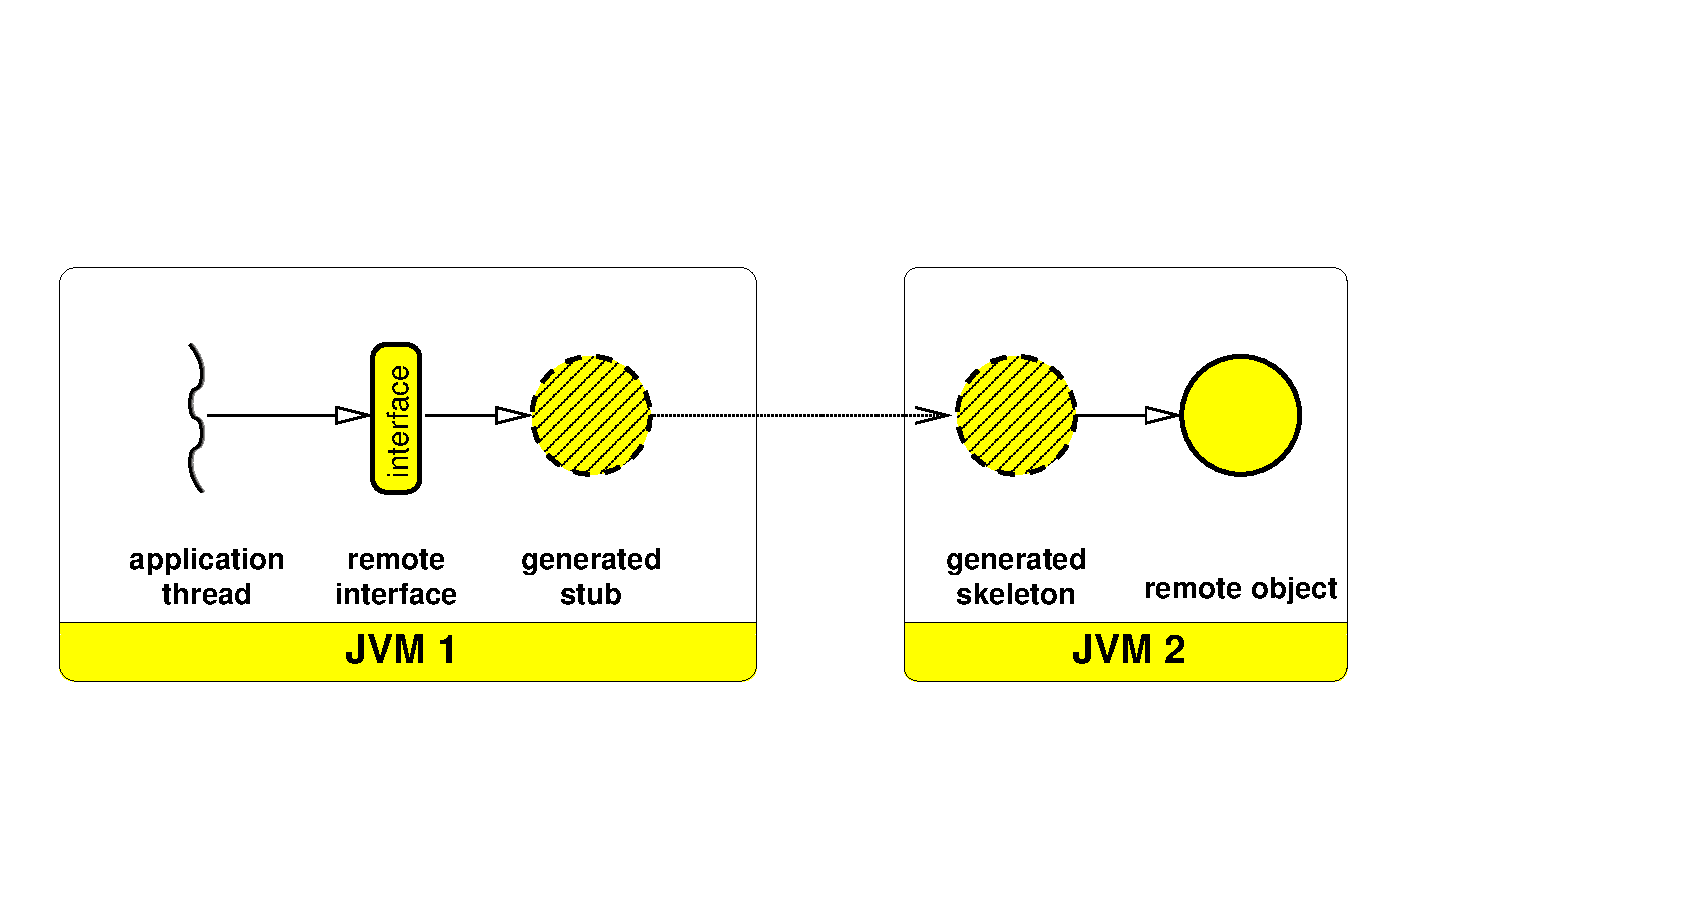
\includegraphics[width=0.7\textwidth]{rmi-abstract.eps}
\end{center}
\caption{A remote invocation with RMI.}
\label{rmi-fig}
\end{figure}

The stub object implements the application interface, and contains
code to forward any method invocations it receives to a skeleton
object on another JVM. The skeleton object contains code to receive
these invocations, and perform them on the object. It then sends the
results back to the stub, which returns them to the waiting
application thread.  Although RMI is not completely transparent, only
small modifications to the application are required. Furthermore, the
programmer does not have to write any communication code (this is
generated by rmic), making RMI easy to use. Unfortunately, the way in
which method invocations are handled in RMI is fixed. After the stub
forwards the invocation to the skeleton, it waits for a reply message
before continuing. The skeleton must therefore always send a reply
back to the stub (even if the method has no result. Furthermore, a
stub in RMI always serves as a 'remote reference' to a single object,
which can not be changed once the stub has been created.

There is very little difference between the usage of Sun RMI and Ibis
RMI. The programs are exactly the same, you only have to compile them
with Ibis \texttt{rmic} instead of the Sun \texttt{rmic}. 

%\remark{TODO limitations/restrictions.}

\mysection{Compiling and running an Ibis RMI program}

Before running an Ibis RMI application it must be compiled.
Using \emph{ant}, this is quite easy. Here is an example build.xml file:

{\small
\begin{quote}
\begin{verbatim}
<project
    name="Project name"
    default="build"
    basedir=".">

    <description>
    Ibis RMI application build.
    </description>

    <property environment="env" />
    <property name="ibis"   value="${env.IBIS_HOME}" />

    <property name="build"  location="build"/>

    <import file="${ibis}/build-files/apps/build-rmi-app.xml"/>
</project>
\end{verbatim}
\end{quote}
}

Again, we assume that the environment variable \texttt{IBIS\_HOME} reflects
the location of your Ibis installation.

Invoking \emph{ant build-sun} compiles a standard Java RMI version of
the application, leaving the class files in a directory called \texttt{build}.
Invoking \emph{ant build} compiles the application for Ibis RMI.
Running an Ibis RMI program is very much like running an Ibis application.

To test this for yourself, it is best to start with
an example, say \texttt{\$IBIS\_HOME/apps/rmi/tsp}. 
If you want to test your own application, it is easiest to just copy
the \texttt{build.xml} file from \texttt{\$IBIS\_HOME/apps/rmi/tsp}, and adapt it for your
application. 
To compile the TSP example, please type

\noindent
{\small
\begin{verbatim}
$ ant clean build-sun
\end{verbatim}
}
\noindent
Now, this example application will be compiled with Sun RMI.
Running the TSP example with Sun RMI can be done as follows. Run the command

\noindent
{\small
\begin{verbatim}
$ java \
    -cp $IBIS_HOME/lib/ibis.jar:$IBIS_HOME/3rdparty/log4j-1.2.9.jar:build \
    -Dibis.pool.total_hosts=2 -Dibis.pool.server.host=localhost \
    Server table_15.1
\end{verbatim}
}
\noindent
in two seperate shells. The application should now run ``in parallel''
on the local machine. Alternatively, you can use the \emph{ibis-run} script:

\noindent
{\small
\begin{verbatim}
$ $IBIS_HOME/bin/ibis-run -nhosts 2 -hostno 0 Server table_15.1
\end{verbatim}
}

\noindent
in the first shell, and

\noindent
{\small
\begin{verbatim}
$ $IBIS_HOME/bin/ibis-run -nhosts 2 -hostno 1 Server table_15.1
\end{verbatim}
}

\noindent in the second.

The TSP application uses the \texttt{PoolInfo}
class that comes with Ibis. This utility class can be used both with
Sun RMI and Ibis RMI. This class is there for convenience, it provides
some methods to retrieve the number of processors in the parallel run
and the ranks of the participating processors. Because this class
comes with Ibis, \texttt{ibis.jar} has to be in the classpath, even
when running with Sun RMI.  The \texttt{PoolInfo} class needs the
\texttt{ibis.pool.total\_hosts} and \texttt{ibis.pool.server.host}
properties in order to be able to assign ranks to processors. The
pool server is started automatically when you start an ibis nameserver
with the \texttt{ibis-namesever} script (in the case of this example, this is done automatically).

Now, we can run the same application with Ibis RMI as follows.
Remember that you first have to recompile it with the Ibis rmic:

\noindent
{\small
\begin{verbatim}
$ ant clean build
\end{verbatim}
}
\noindent
Now we can run it by typing the following command in two seperate shells:

\noindent
{\small
\begin{verbatim}
$ java \
    -cp $IBIS_HOME/lib/ibis.jar:$IBIS_HOME/3rdparty/log4j-1.2.9.jar:build \
    -Dibis.pool.total_hosts=2 -Dibis.pool.server.host=localhost \
    -Dibis.registry.host=localhost -Dibis.registry.pool=bla \
    Server table_15.1 
\end{verbatim}
}
\noindent

This should produce the same result as the Sun RMI test.
If you want to run the application with the \texttt{ibis-run} script,
you can use the same commandline as with the Sun RMI test.

If, for some reason, it is not convenient to use \emph{ant} to compile
your application, or you have only class files or jar files available
for parts of your application, it is also possible to first compile
your application to class files or jar files, and then process those
using the \emph{ibisc} script. This script can be found in the Ibis
bin directory. It takes either directories, class files, or jar files
as parameter, and processes those, possibly rewriting them. In case
of a directory, all class files and jar files in that directory or
its subdirectories are processed.
To process an RMI application, \emph{ibisc} needs to know that it has to
do so.  This can be accomplished by passing either the \texttt{-rmi}
or the \texttt{-rmi-java2ibis} flag to \emph{ibisc}. The latter instructs
\emph{ibisc} to not only use the Ibis rmic, but also to change all
references to \texttt{java.rmi} into references to \texttt{ibis.rmi}.

